\chapter{実験1}
\section{データセット \label{sec:ch2:dataset}}
実験に用いるデータセットとして,
IMDB-wikiデータセット
\cite{Rothe-ICCVW-2015,Rothe-IJCV-2018,imdb-wiki}を用いた.
このデータセットは(主に海外の)映画やドラマの
情報をまとめているオンラインデータベースであるIMDbと
オンラインの百科事典であるWikipediaに含まれる顔写真を
人名や性別,年齢などのタグをつけてデータセット化したものである.
今回の作成するシステムは,入力対象の顔写真を
男性に限定している.そこで,性別情報の含まれるデータセットを利用した.

IMDB-wikiデータセットは自動的にWeb上の情報から
各画像にタグをつけているため,そのタグが必ずしも
正確であるとは限らない.また,
Wikipediaのデータに関しては一部に破損がある問題も存在する.

そのため,今回の実験ではIMDbのデータのみを利用することにし,
そのデータをさらにクリーニングすることにした.
IMDbに含まれる顔写真は主に女優・俳優のものになる.

データのクリーニングは以下の手段で実行した.
\begin{enumerate}
  \item 性別タグが男性であるものを抽出する
  \item IMDb-wikiに含まれる,AIによる顔検出スコアの上位2000件を抽出する.
  \item 名前情報を用いて,同一人物の写真を顔検出スコアが最も高いもの以外削除する.
  \item 目視による手動作業で,タグミスによる女性の写真,複数人が
  写っているもの,白黒写真を除外した.
\end{enumerate}
結果,1076件の異なる男性の顔カラー写真が抽出できた.

\section{クラウドソーシングの実施}
IMDB-wikiデータセットから抽出した顔写真に対して,
クラウドソージングによってワーカーに印象(impression)ラベルを
付与していただき,実験に用いるデータセットとする.

クラウドソージングにはAmazon Mechanical Turk (AMT,mTurk)を利用した.
これは,IMDbが主に海外の映画・ドラマを対象にしていることや,
システムで用いる7つの印象が英語の印象(impression)であることを考慮し,
主にアメリカ人がワーカーとして活動している
\footnote{
2010年の研究では
ワーカーはアメリカ人が約6割,インド人が約3割と
報告されている\cite{10.1145/1753846.1753873}.
現在はその比率も大きく変化しているとも考えられ,
AMTのワーカーが主にアメリカ人であると仮定するのは
誤っている可能性も高い.
}AMTを利用することが最適であると
考えたためである.

\subsection{タスクインストラクション}
AMTを用いて,画像に対して複数の印象を選択する
クラウドソージングタスクを作成した.
図\ref{fig:ch2:task}にタスクのスクリーンショットを示す.
\begin{figure}[tb]
  \centering
  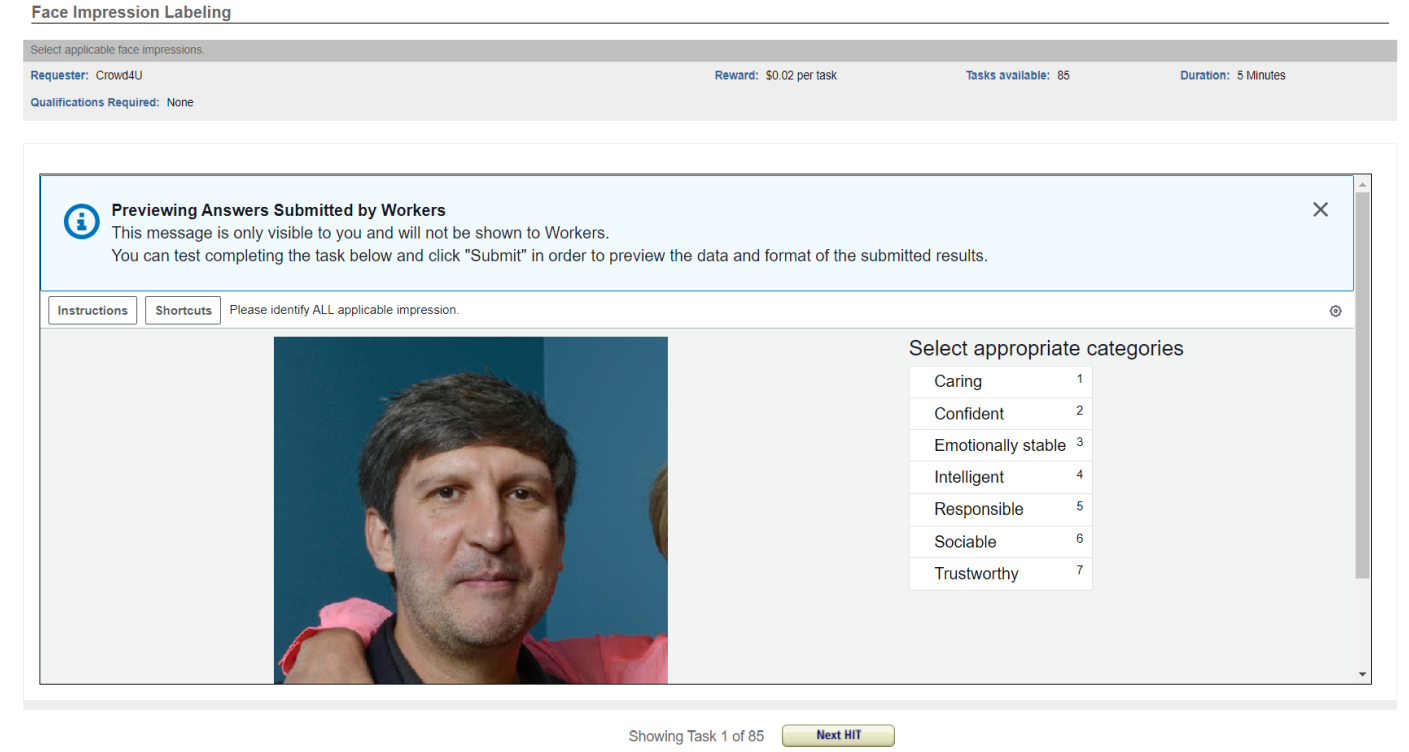
\includegraphics[width=12cm]{ch2/task.png}
  \caption{
  クラウドソージングタスクのスクリーンショット
  \label{fig:ch2:task}
  }
\end{figure}
タスクの説明などは以下のように設定した.
\begin{itemize}
  \item Project Name: Face Impression Labeling
  \item Title: Select applicable face impressions.
  \item Description: Please identify ALL applicable
  face impression labels with the given photo.
  You can select multi labels each photo, if you
  think several labels match the face.
  \item Keywords: categorize, image
\end{itemize}

AMTでは画像に対して複数のタグを選択させる場合,
crowd-image-classifier-multi-selectを用いることができる.

\subsection{人数・値段・工夫した点}
以下のように人数・値段を設定した.
\begin{itemize}
  \item 1タスク3ワーカー
  \item 1タスク当たりのワーカー報酬は\$0.02
  \item 1タスク当たりのAMT手数料は\$0.01
  \item 85タスク実施
\end{itemize}
よって
請求金額は,
85タスク$\times$3ワーカー$\times$\$0.03$=$\$7.65となった.
タスク数85は1000円という予算を考慮して決定した数である.
1タスクあたり3秒と見積もっており,
時給換算すると\$24となる.これは
インフレを考慮しても,アメリカの最低賃金
を大幅に上回る額であると考えられる.

\ref{sec:ch2:dataset}節で抽出した顔写真のうち,
顔検出スコアの高い85枚を抽出し,
筑波大学全学計算機システムWeb公開サービスを用いて
タスクに埋め込んだ.

クラウドソージングタスクを作成するのは初めてだったので,
勉強を兼ねて,1タスクあたりのワーカー数を3に設定し,
結果の多数決による統合などを試してみることにした.
3は多数決を行える最も小さい数値である.

誤って男性とタグ付けされている写真を削除するなど.
あらかじめデータセットをクリーニングしておいたことで,
無意味なタスクを実行してしまう可能性を下げることが
できたと考えられる.これはクラウドソーシングを
行う上で工夫した点の一つである.

\section{クラウドソーシングの結果}
AMTでクラウドソーシングを行い,
85タスク$\times$3ワーカー$=255$件のデータを得た.

\subsection{ワーカーあたり回答数の分布}
\begin{figure}[tb]
\centering
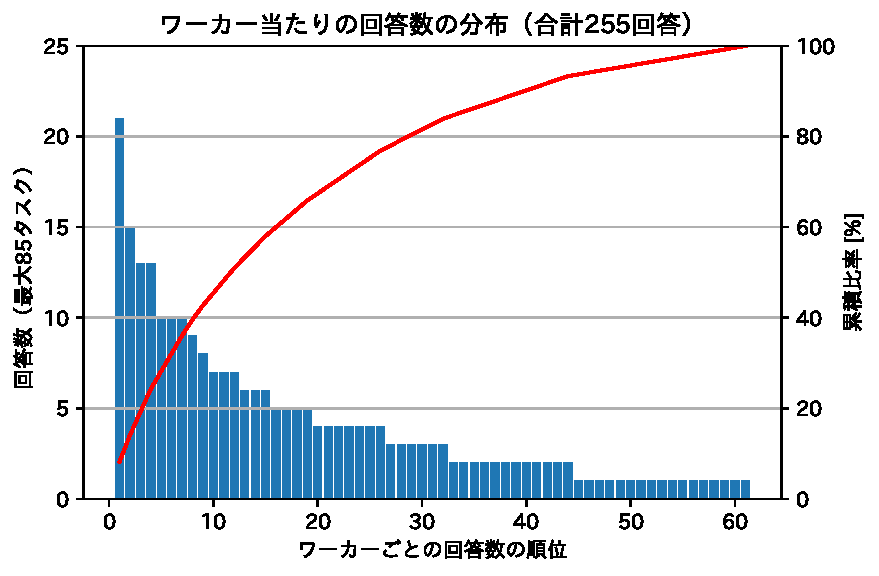
\includegraphics[width=10cm]{ch2/worker_plot.pdf}
\caption{ワーカー当たりの回答数の分布(パレート図)
\label{fig:ch2:worker}}
\end{figure}
クラウドソーシングには61人のワーカーが
参加した.
ワーカー当たりの回答数の分布をパレート図にしたものを
図\ref{fig:ch2:worker}に示す.
これを見ると,1/6のワーカーが,
全体の50\%を回答していることがわかる.

AMTでは,1ワーカーあたりが回答できるタスク上限数を
設定することができないため,このように,
一部のワーカーが多くを回答することがある.

\subsection{クラウドソーシング結果の統合}
実験1のクラウドソーシングでは,
1タスクを3ワーカーが担当した.
そこで.その結果を多数決などの手法により
統合する必要がある.

マルチクラス問題とは異なり,
マルチラベル問題の場合,
結果の統合手法は十分に研究されていない.
そこで,いくつかの方法を考え,
最適そうな手法を採用することにした.

\subsubsection{ラベルごと単純多数決}
マルチクラス問題における単純多数決では,
各ワーカーの回答の中で最も数が多い回答を選択する.

しかし,マルチラベル問題では回答
がワーカー間で完全に一致することは少なく,
完全に一致する回答数をカウントすることはナンセンスである.

そこで,ラベルごとにワーカー間で多数決を取り,
その結果を統合した回答として,
ラベルごとの単純多数決とした.

\begin{figure}[tb]
  \centering
  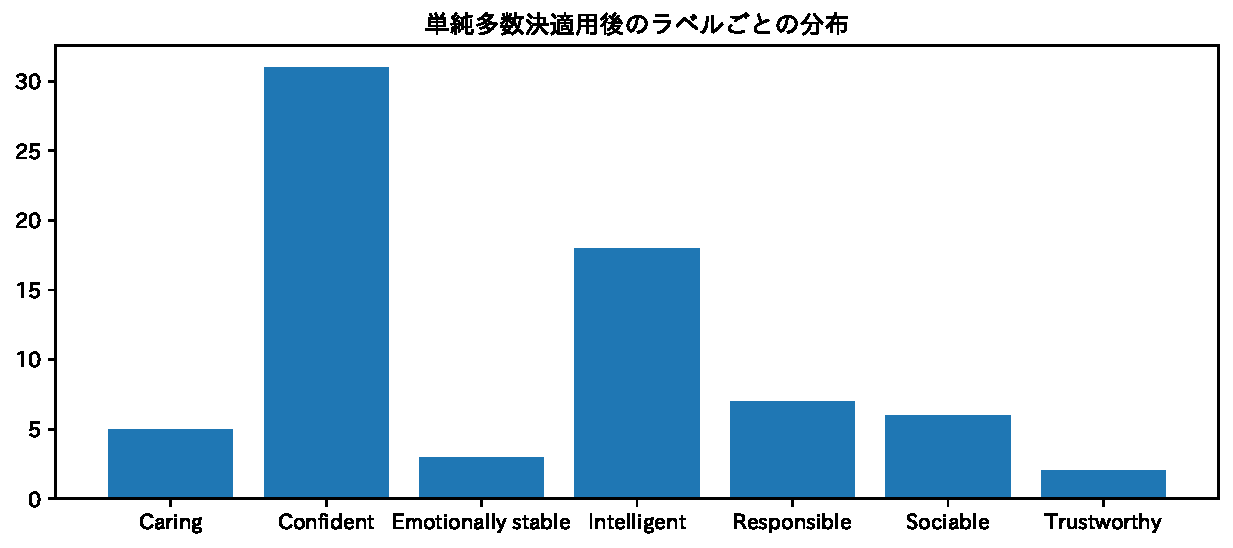
\includegraphics[width=10cm]{ch2/smv_plot.pdf}
  \caption{ラベルごと単純多数決を適用した際のラベル数の分布
  \label{fig:ch2:smv}}
\end{figure}

図\ref{fig:ch2:smv}にラベルごと単純多数決を適用した場合の
ラベル数の分布を示す.
これを見ると,ラベルごと単純多数決では,
いくつかのラベルにおいて,
そのラベルが割り当てられた画像数が
極端に少なくなってしまっている.

極端に不均衡なデータに対して,
機械学習を適用することは難しい.
実際に,機械学習を適用した際には,
単純多数決のデータはうまく機能しなかった.

\subsubsection{和集合}
そこで,単純多数決以外の手法として,
和集合という手法を考えた.

これは,各ワーカーが付与したラベルの集合を考え
,その3集合の
和集合を統合した回答とするものである.
言い換えれば,これは
1人でもラベル付けしたものは有効とし,
統合結果に反映するものである.

\begin{figure}[tb]
  \centering
  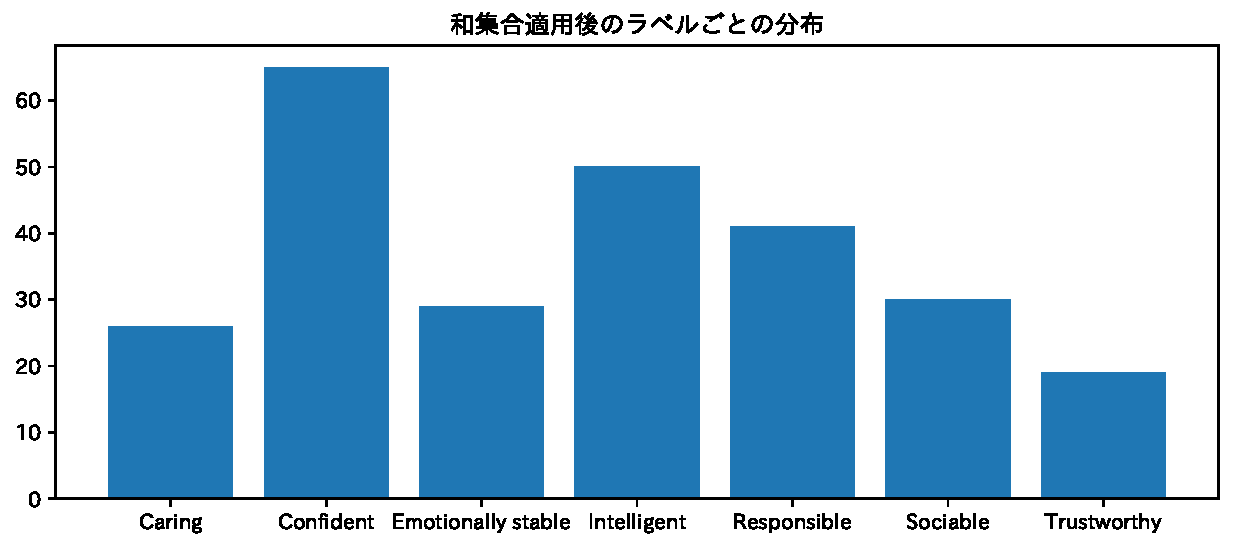
\includegraphics[width=10cm]{ch2/svs_plot.pdf}
  \caption{和集合を適用した際のラベル数の分布
  \label{fig:ch2:svs}}
\end{figure}

図\ref{fig:ch2:svs}に和集合を適用した場合の
ラベル数の分布を示す.これを見ると,
単純多数決の時よりも,ラベル数の不均衡さが
改善していることがわかる.

単純多数決を採用したほうが理論的には正しい
と考えられる.しかし,単純多数決のデータは
極端に不均衡であり,機械学習を行うのに適していない.
そこで,苦肉の策として,和集合のデータを採用することにした.

\section{機械学習の実施}
\subsection{環境}
機械学習を行うソフトウェア・ハードウェア環境について述べる.
機械学習の実行は自宅のPCを用いた.
\subsubsection{ソフトウェア}
今回のテーマは画像を扱うものであり,
機械学習手法には深層学習を用いる.
そのために,Pythonに加えて,深層学習ライブラリ
TensorFlow
を利用した.
\begin{itemize}
  \item OS: Windows 11 64bit
  \item Python 3.9
  \item TensorFlow 2.8
  \begin{itemize}
    \item CUDA 11.2
    \item cuDNN SDK 8.1.0
  \end{itemize}
  \item Jupyter Notebookを利用
\end{itemize}
また,各種疑似乱数の種は$1001$に設定した.
\subsubsection{ハードウェア}
\begin{itemize}
  \item CPU: AMD Ryzen 5 3600
  \item GPU: NVIDIA GeForce RTX 3060
\end{itemize}
GPUを用いて計算を行った場合,
毎度微妙に計算結果が変わり,
再現性に若干の問題が生じることがある.
\subsection{前処理}
画像データに対する前処理として,
FaceNet\cite{Schroff_2015_CVPR}を利用した.
FaceNetは顔写真データをベクトル空間に埋め込める
機械学習アルゴリズムであり,学習済みモデルを用いることで,転移学習のように
用いることができる.
FaceNetは顔認証システムなどに用いられており,
顔写真から特徴量を抽出するには適したモデルである,

今回はインターネットで公開されている
VGGFace2モデルのバージョン20180402-114759\cite{face-net}を
を利用し,すべての顔写真データを512次元のベクトルに変換した.
\subsection{機械学習モデル}
マルチラベル問題では,2値分類を行う機械学習モデルを
ラベル数分用意し並列して動作させる手法と,
1つのモデルでマルチラベル問題を解く手法の
2手法が考えられる.今回は両手法を共に実装し,その性能を比較した.
以降,前者を二値分類モデル,後者を
マルチラベルモデルと呼称する.

\subsubsection{モデルのハイパーパラメータ}
機械学習モデルにはDNN(Deep Neural Network)を用いる.
モデルの構造を表\ref{tab:ch2:model}に示す.
出力層を除いて,両者のモデル構造は共通しており,
隠れ層の活性化関数にはReLUを使用した.
入力層にはFaceNetにより前処理された
512次元のベクトルを入力する.
また,モデルには過学習を防ぐための
Dropout層を追加している.
\begin{table}[tb]
  \caption{DNNモデルの構造
  \label{tab:ch2:model}}
  \centering
  \begin{tabular}{c|cc}
  \hline
  層種       & ニューロン数 & 比率  \\ \hline
  入力層      & -      & -   \\
  全結合層     & 512    & -   \\
  全結合層     & 1024   & -   \\
  Dropout層 & -      & 0.4 \\
  全結合層     & 1024   & -   \\
  Dropout層 & -      & 0.4 \\
  全結合層     & 512    & -   \\
  全結合層     & 256    & -   \\
  全結合層     & 128    & -   \\
  Dropout層 & -      & 0.2 \\
  出力層      & 2 or 7 & -   \\ \hline
  \end{tabular}
\end{table}

出力層は,二値分類モデルでは
ニューロン数を2とし,活性化関数にsoftmax関数を用いた.
softmax関数は確率を出力するものであり,
出力層の全出力の和が1となるように設計されている.
そのため,マルチラベルモデルにおいてsoftmax関数を
用いることはできない.ゆえに,
マルチラベルモデルの出力層には,
活性化関数にsigmoid関数を利用し,
ニューロン数をラベル数である7とした.

両モデルともに損失関数には二値交差エントロピー
(binary crossentropy)を用いた.

\subsubsection{学習の実行}
はじめに,学習と検証には
3分割交差検定法(3-fold Cross Validation)
を用いた.

二値分類モデルでは,不均衡データに対応しやすくするための
TensorFlowのハイパーパラメータである
class\_weights\cite{unbalanced-data}を
学習データのラベルの有無比率に応じて設定した.
これは損失関数に重み付けを与えるものである.

二値分類モデルでは学習回数を6,
対して,マルチラベルモデルでは,学習回数を10とした.
また,両モデル共にミニバッチ法のバッチサイズを8とし,
最適化法にはAdamを用いた.

\subsection{評価指標}
評価指標には,
\begin{enumerate}
  \item ラベルごとのF1-score
  \item macro-F1
  \item Hammig Loss
\end{enumerate}
を用いる.
\subsubsection{F1-score}
あるラベル$l$における,
真陽性($TP$),偽陽性($FP$),
真陰性($TN$),偽陰性($FN$)の数を考えた時,
適合率と再現率,すなわち,
\begin{align*}
  \mathrm{Precision} = \frac{TP}{TP+FP} \\
  \mathrm{Recall} = \frac{TP}{TP+FN} 
\end{align*}
が定義できる.
ここで,あるラベルの$l$のF1-scoreは,
\begin{align*}
  \mathrm{F1}_l = \frac{2\times \mathrm{Precision} \times 
  \mathrm{Recall}}{\mathrm{Precision} + \mathrm{Recall}}
\end{align*}
で与えられる.F1-scoreは0から1の値を取り,
1に近づくほど良いモデルであるといえる.
\subsubsection{macro-F1}
$L$をすべてのラベルの集合として,macro-F1
は以下のように定義される.
($\# L$は$L$の元の数,すなわち7である.)
\begin{align*}
  \mathrm{macroF1} = \frac{1}{\# L} \sum_{l \in L} \mathrm{F1}_l
\end{align*}
すなわち,macro-F1はラベルごとのF1-scoreの平均値である.
\subsubsection{Hamming Loss}
今回のマルチラベル問題では,
1つの画像につき,7つのラベルの有無を確認する.
ここで,1つの画像に対する正解データを,
1がラベルあり,0がラベル無しとすると,
タプルを用いて$(1,0,0,1,0,1)$のように表現することができる.
予測データと正解データをこの形式で表現し比較した時,
数値が異なる要素の数をタプルの長さで割ったものを考える.

例えば,正解$(1,0,0,1,0,1)$に対して,予測
$(1,0,0,1,1,0)$であれば,異なるビット数は2,
タプルの長さは7であるから,$2/7 = 0.286$のように考える.
この値をすべての検証データで計算し,その平均を取ったものを
Hamming Lossという.

正確な定義では,Hamming Lossは0と1でのみ構成される
2つの$m \times n$行列において,$(i,j)$要素が一致しない
数を$mn$で割った数である.
\subsubsection{なぜ評価指標にこれらを用いるのか}
マルチラベル問題では,適切な評価指標を設定する
ことが難しい.
例えば,今回のシステムにおいては,
予想が正解と完全に一致しない場合は不可とするような,
つまり,1つの検証データに対するHamming Lossが
0になるようなデータのみを正解とする
とするのはナンセンスである.

F1-scoreは優れた評価指標であるが,不均衡なデータに対しては
不適切であることもある.適合率と再現率の分子が$TP$であるために,
すべてをラベルありと分類したほうがF1-scoreは高くなってしまうことがある.

対して,Hammig Lossは厳密な損失であり,1つでも
予想と正解が異なれば損失の値は大きくなる.
代わりに,Hamming Lossは比較的不均衡なデータに強いのではないかと
予想される.

それゆえに,今回はこの3種を評価指標として
併用することにした.
\section{機械学習の結果}
両モデルにおいて,機械学習を行った結果を,
図\ref{fig:ch2:result}に示す.

\begin{figure}[p]
  \centering
  \subfloat[二値分類モデルの結果]
  {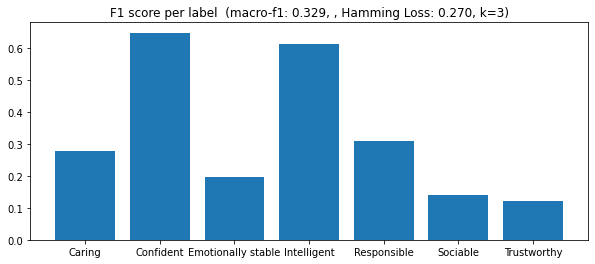
\includegraphics[width=12cm]{ch2/binary.png}
  \label{fig:ch2:binary}}
  \\
  \subfloat[マルチラベルモデルの結果]
  {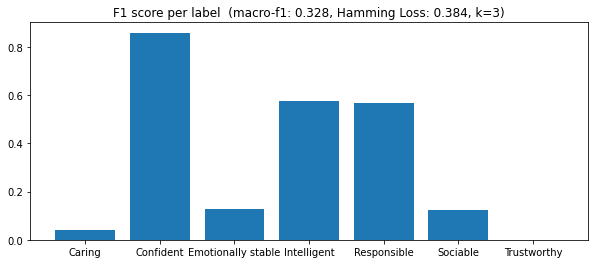
\includegraphics[width=12cm]{ch2/multi.png}
  \label{fig:ch2:multi}}
  \caption{ k=3でk分割交差検定法を実施した結果.\\
    各ラベルにおけるF1-score (棒グラフ)と
  そのmacro-F1ならびにHamming Loss (グラフタイトル).
 }
  \label{fig:ch2:result}
\end{figure}

これを見ると,まず,両モデルでmacro-F1に大きな差はなく,
その値が0.3程度であることがわかる.F1-scoreは0.8程度で
あることが望ましく,機械学習は両モデルともうまくいっていないことがわかる.

Hammig Lossに関しては,二値分類モデルのほうが小さい.
また,ラベルごとのF1-scoreを見ても,二値分類モデルのほうが,
各ラベルのバランスが取れているように見受けられる.
例えば,マルチラベルモデルでは,ラベルtrustworthyの
F1-scoreが0になってしまっているなど,いくつかのラベルで
極端にF1-scoreが低い.
これは,データが不均衡であるために,
機械学習モデルがすべてのデータをラベルあり,あるいは,
ラベルなしと予測してしまっていることが原因である.
その点から,二値分類モデルのほうがやや「マシである」と
考えることができる.

機械学習がうまくいかなかった理由としては,
データ総数が85と,少なすぎたことが考えられた.
データ数85で3分割交差検定法を用いた場合,
trustworthyなどの特に不均衡なラベルでは
テストデータ内でラベルの付いた画像数が0や1と
なってしまうこともあった.その場合,
F1-scoreの値は正常なものとは言えないだろう.

中間発表のフィードバックでは,
k分割交差検定法ではなくLeave One Out Cross Validation
(LOOCV)の利用について助言を受けた.
また,
データ数を増やすために2回目のクラウドソージンングを
行うことを決めた.その過程については,次章で記述する.
\section{機械学習の上手くいかなかった例}
実験1の機械学習は最終的にうまくいっていないものの,
様々な試行錯誤の中ではもっともうまくいった手法であった.
この節では,その試行錯誤について,少しだけ説明する.

\subsection{前処理}
\subsubsection{imagenetの利用}
imagenetを事前学習したVGG16モデルによる
転移学習・ファインチューニングを試したが,
imagenetは顔の特徴抽出に最適化されていないため,
FaceNetよりも精度が低かった.
\subsubsection{Data Augmentation / Over Sampling}
Data Augmentationとは不均衡なデータに対して,
行われる前処理手法の一つである.
少ないラベルのデータに加工を施しデータを複製し,
データを水増しすることでデータを均衡なものとする.
Over Samplingともいう.画像データであれば画像を傾ける,色合いを変える
などとしてデータを水増しすることになる.

Data Augmentationは便利な手法であるが,
データを複製して水増しするため,過学習のリスクも大きい.
今回の実験1ではあまり効果はなかったため,
採用しなかった.
\subsubsection{Under Sampling}
また,Over Samplingとまったく逆の発想として,
ラベル数の多いデータを削減し,不均衡さを軽減する
Under Samplingという手法もある.
しかし,これを行うとただでさえ少ない85という
データ数がさらに少なくなってしまい,
機械学習を行うことが困難になる.
そのため,今回の用途では利用できなかった.
\subsection{機械学習手法}
\subsubsection{DNN以外の手法の利用}
DNNではなくLightGBM(Light Gradient Boosting Machine)
といった機械学習手法も試してみたが,
DNNのほうが複雑な手法であり,精度が高かった.
\subsubsection{損失関数のカスタマイズ}
損失関数は二値交差エントロピー(binary crossentropy)
ではなく,F1-scoreに変更することもできる.
その場合,F1-scoreに機械学習結果が最適化されるため,
結果が改善されることが見込まれたが,
先述したように,
F1-scoreは不均衡なデータに対して正常に機能しない
ため,より精度が悪化する結果となった.